\documentclass[a4paper]{article}

\usepackage{listings}
\usepackage{color}
\usepackage{graphicx}

\usepackage[top=2.0cm, bottom=2.0cm, left=2.0cm, right=2.0cm]{geometry}

\begin{document}

\title{Embbeded Systems - Exercise 02}

\author{Jander Nascimento \and Luka Stanisic}

\maketitle

\section{Question 1}

\subsection*{a)}

$
AG(AF p \to AF q) \Rightarrow
\newline AG (\neg AF p \lor AF q) \Rightarrow
\newline AG( \neg \neg EG \neg p \lor \neg EG \neg q ) \Rightarrow
\newline \neg EF ( \neg EG \neg p \land EG \neg q )
$

\subsection*{b)}

$
AF(p \lor AG q) \Rightarrow
\newline AF (p \lor \neg EF \neg q) \Rightarrow
\newline \neg  EG \neg (p \lor \neg EF \neg q) \Rightarrow
\newline \neg EG (\neg p \land  EF \neg q)
$

\section{Question 2}

\subsection*{a)}
Looking at $EG$ it means that should exist at least one path in the whole set of paths in which $p$ hols in the entire path. 
At the picture in the exercise the only path that follows that is the $a \to a \to a ...$, in this particular path $p$ holds all the way long. So the statement is \textbf{true} for the Kripke structure. 

\subsection*{b)}
%By dissecting $AG EF p$ we can say that, it requires that all subpaths generated from the initial path holds p, which is not \textbf{true} in this case. $P$ holds just in the case of subpath mentioned in the last answer($a$)

By splitting the expression $ AG \quad EF \phi $ we have: $ EF $ ensures that $ \phi $ holds in at least one state in the paths. $AG \omega $ means that $ \omega $ must be reachable from every single state in all paths.

So the statement $AG \quad EF p $ does \textbf{NOT} hold, since if we start from the state $A$ we can get only $p$ (if we get in the loop).

\subsection*{c)}

We can derivate $E \quad true \quad U (\neg ( E \quad true \quad U \quad p ))$ ($\gamma$) from $AG \quad EF \quad p$ ($\sigma$) (Equation \ref{equa:e1}).

\begin{equation}
AG \quad EF \quad p \Rightarrow \newline
AG \quad E \quad true \quad U \quad p \Rightarrow \newline
\neg EF \quad \neg ( E \quad true \quad U \quad p ) \Rightarrow \newline
E \quad true \quad U (\neg ( E \quad true \quad U \quad p ))
\label{equa:e1}
\end{equation}
 
We can solve the equation per block, starting from $\alpha=E\quad true \quad U \quad p$.

$
E\quad true \quad U \quad p=\mu Z. p \lor (p \land EX Z) \Rightarrow \newline 
Z_0=\emptyset; \newline
Z_1=p \lor ( true \land EX Z_0 ) \Rightarrow \{a,c\} \cup (true \cap  Z_0) = \{a,c\} ; \newline
Z_2=\{a,c\} \cup ( true \cap \{a,b\} = \{a,b,c\} \newline
Z_3=\{a,c\} \cup ( true \cap  \{a,b,c\} ) = \{a,b,c\} \newline
$

By applying in the initial formula we have:
$
T_0=E \quad true \quad U (\neg ( \alpha )); \newline
T_1=E \quad true \quad U (\neg ( \{a,b,c\} )); \newline
T_2=E \quad true \quad U (\emptyset); \newline
T_3=\emptyset;
$ 

So the statement does \textbf{NOT} hold in the given Kripke structure.

\section{Question 3}

\subsection*{a)}

If in $EF ( p \lor q ) $ one or the terms ($p$ or $q$) are satisfied that means that $p$ or $q$ are present in at least one state of the path, which can be interpret as $EF p \lor EF q$.

So, this statement is \textbf{True}.

\subsection*{b)}

From the image below (Figure \ref{fig:3b}), we can see two possible paths ($a \to a$ and $a \to b$), This tree is complaint with $EF p \land EF q$ but NOT with $EF ( p \land q )$.

\begin{figure}[h]
		\centering
		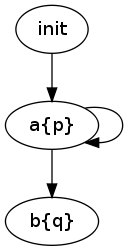
\includegraphics[scale=0.50]{img/3b}
		\label{fig:3b}
\end{figure}

So, this statement is \textbf{False}.

\subsection*{c)}

According to definition given by this model, $EG \phi $ requires that eventually the state $\phi$ be reached in every path at least once. 

If we evaluate $EG (p \lor q)$, its valid since we have a path that respect that requirement, which does not happen with 
$EG p \lor EG q$.

\begin{figure}[h]
		\centering
		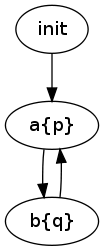
\includegraphics[scale=0.50]{img/3c}
		\label{fig:3c}
\end{figure}

So, this statement is \textbf{False}.

\subsection*{d)}

MISS

%this must be true :-S just do know how prove that

\subsection*{e)}

MISS

%this is true, how prove?

\section{Question 4}

$EG p$ is a fix-point of $f.Z = p \land EX(Z)$ because $f.EG p = p \land EX EG p=EG p$ holds.

$EG p$ is greatest fix-point since the states satisfying $EG p$ are: $EG p=\land i >= 0EX_{i}p$

Considering arbitrary fix-point $F$ of $\lambda Z.p \land EX Z$ since $F=p \land EX F$, we know $F \leq EX F$ and $F \leq p$. Since $EX$ is monotone $( x \leq y \to EX(x) \leq EX(y))$, we get by induction over $i \geq 0$ that for all $i \geq 0: F \leq EX_i F$ holds, and $F \leq \land_{i \geq 0} EX_iF=EG F$. From $F\leq p, F\leq EG, F\leq EG p$. So $EG p$ is greater then or equal to any arbitrary fix-point - $EG p$ is the greatest fix-point.

\section{Question 5}

First we assume that we have a Kripke structue with \textit{n} states. Now lets assume that $EG p=X$, where $X$ is a set with \textit{l} number of states. So now we have to prove that $EG X=X$:

\[
EG X = \upsilon Z.X \land EX Z 
\] we have: 


$
Z_0=S=\{s_0,s_1,s_2,...s_n\} \\
Z_1=X \land EX Z_0 = \{s_0,s_1,s_2,...s_l\} \land EX S = \{s_0,s_1,s_2, s_l\}=X \\ 
Z_2=X \land EX Z_1= \{s_0,s_1,s_2...s_l\} \land EX X = \{s_0,s_1,s_2,... s_l\}=X \\
$

So $X$ is a fix-point, which means that the equation is correct $EG EG p = EG p$

 
\section{Question 6}

For $E p U q= \mu Z. q \lor p \land EX Z $, having:

$Z_0=\emptyset $

$Z_1=q \lor (p \land EX Z_0)=\{c\} \lor (\{ b, d \} \land \emptyset)=\{c\} $

$Z_2=q \lor (p \land EX Z_1)=\{c\} \lor (\{b, d\} \land \{b\})=\{b,c\} $

$Z_3=q \lor (p \land EX Z_2)=\{c\} \lor (\{b, d\} \land \{a, b\})=\{b,c\}=¨fix-point¨   $

\section{Bonus}

\subsection*{a)}

Since $Z_i = q \lor X$, where $X$ could be any set including empty set, we always apply unions so our result is monotonically getting bigger in every step. $Z_{i+1}$ can only be bigger than $Z_i$. Since the set $S$ is the hole set, meaning there is no bigger set than $S$, when $Z_i$ reaches $S$ it cannot grow more in next iteration and it will certainly not get any smaller, hence the $S$ is a fix-point.

\subsection*{b)}

Since $Z_i=q \lor (p \land X)$, where $X$ could be any set including the hole set, the result in the brackets can in maximum be $p$, because we are doing intersection. Hence the maximum set could only be $q \lor p$, and since the size of the result is monotonically rising as proved in the previous example, this is a fix-point. 

\subsection*{c)}

$Z_0=\emptyset$

$Z_1=q \lor ( p \land \emptyset )=q$

%\newline 
So all the states where $q$ is correct are added at the beginning and they will stay in the resulting set. As proved in the previous example, the set in the brackets can be in maximum $p$, which means that when we reach the $Z_i \geq p$, it cannot get any bigger, so its a fix-point.

\end{document}
